\documentclass{report}

\usepackage{adjustbox}
\usepackage[intlimits]{amsmath}
\usepackage{mathtools}
\usepackage{nonfloat}
\usepackage{amsmath}
\usepackage{adjustbox}
\usepackage{setspace}
\usepackage[paperwidth=16cm,paperheight=24cm]{geometry}
\usepackage[a4,frame,center]{crop}

\graphicspath{{/home/abhishek/Desktop/"Text Classification"/Report/figures/}}
%\graphicspath{{/home/ayush/Downloads/project/LATEX_project_report/extras/}}
\usepackage{lipsum}% dummy text
\usepackage[titles]{tocloft}

\setlength\cftbeforechapskip{100pt}
\renewcommand\cftfigafterpnum{\vskip10pt\par}
\renewcommand\cfttabafterpnum{\vskip10pt\par}


\usepackage{url}
\usepackage{tocloft}
\usepackage{enumitem}
\usepackage{chngcntr}
\usepackage[svgnames]{xcolor}
\usepackage{pgfplotstable}
\usepackage{pgfplotstable,booktabs}
\usepackage{csvsimple}
\usepackage{multicol}
\usepackage[pdfpagemode=FullScreen, colorlinks=true]{hyperref} 
\usepackage{hyperref}
\hypersetup{%
  colorlinks = false,
  linkcolor  = black
}
\usepackage{graphicx}
\usepackage{subcaption}
\usepackage{filecontents}
\newcommand{\plogo}{\fbox{$\mathcal{PL}$}}
\usepackage[utf8]{inputenc}
\usepackage[T1]{fontenc}
\usepackage{fouriernc}
\usepackage[utf8]{inputenc}
\usepackage{titlesec}
%\usepackage{etoolbox}
%\makeatletter
%\patchcmd{\ttlh@hang}{\parindent\z@}{\parindent\z@\leavevmode}{}{}
%\patchcmd{\ttlh@hang}{\noindent}{}{}{}
%\makeatother
\usepackage{titletoc}
\usepackage[figurename=Fig - ]{caption}
\usepackage[tablename=Table - ]{caption}

\usepackage{geometry}
 \geometry{
 a4paper,
 tmargin=25mm,
 bmargin=20mm,
 left=20mm,
 right=20mm,
 top=20mm,
 }

\renewcommand\thesection{\arabic{section}}
\titlecontents{chapter}[1.05em]{\bigskip}%
{\contentslabel[\MakeUppercase{\romannumeral\thecontentslabel}]{1em}\enspace\textsc}%numbered\contentslabel
{\hspace*{-1em}\textsc}%numberless
{\hfill\contentspage}%
%
\titlecontents{section}[1.6em]{\bigskip}%
{\thecontentslabel.\enspace}%numbered
{}%numberless
{\titlerule*[1pc]{.}\contentspage}%

\setcounter{tocdepth}{6}

\usepackage{lipsum}

\newcommand\myfigure[1]{%
\medskip\noindent\begin{minipage}{\columnwidth}
\centering%
#1%
%figure,caption, and label go here
\end{minipage}\medskip}


\newenvironment{changemargin}[1]{%
\item[]}{\end{list}}
\setlength{\columnsep}{0cm}

\begin{document} 
\begin{titlepage}
	\centering
	
\includegraphics[width=4cm]{logo.png}\\[.5cm]
	{\scshape\LARGE Indian Institute of \\Information Technology, Allahabad \par}
	\vspace{1cm}
	\rule{\textwidth}{2pt}	
	%\vspace{2pt}\vspace{-\baselineskip}
	%\rule{\textwidth}{0.4pt}
	\vspace{0.1\textheight}
		
	\textcolor{Red}{ 
		{\fontsize{35}{42}\selectfont Text Classification}\\[0.5\baselineskip]
		{\fontsize{24}{28.8}\selectfont Using}\\[0.5\baselineskip]
		{\fontsize{35}{42}\selectfont Support Vector Machine}
	}
	
	\vspace{0.155\textheight} 
	
	\rule{0.3\textwidth}{0.4pt} 
	\begin{multicols}{3} 
	\textcolor{Blue}{
		\begin{flushleft} 
		{\large Ayush Agnihotri}\\[5pt] 
		{\large Nidheesh Pandey}\\[5pt]
		{\large Abhishek Pasi}\\[5pt]
		{\large Shreyansh Gupta}\\[5pt]
		{\large Vishal Kumar Singh}\\[5pt]
		\end{flushleft}
		}
		\columnbreak
		 
	\textcolor{Blue}{
		\begin{flushleft} 
		{\large IIM2015004}\\[5pt] 
		{\large IIM2015501}\\[5pt]
		{\large ICM2015002}\\[5pt]
		{\large IIM2015001}\\[5pt]
		{\large IIT2015141}\\[5pt]
		\end{flushleft}
		}
		\columnbreak

	\textcolor{Green}{
		\begin{flushright}
		{\Large \textsc{Under supervision}}\\
		{\large of}\\
		{\Large \textsc{\textbf{Dr. K P Singh}}}
		\end{flushright}
		}
	\end{multicols}
	
\hfill
		
	\rule{\textwidth}{0.4pt} % Thin horizontal rule
	
	\vspace{2pt}\vspace{-\baselineskip} % Whitespace between rules
	
	\rule{\textwidth}{2pt} % Thick horizontal rule
	
\end{titlepage}
\pagebreak
{\section*{ \quad \quad \quad \quad \quad \quad \quad \quad \quad \quad \quad \quad  \Huge \scshape Declaration}
\vspace{2.0cm}
\ \ \ \ \LARGE We hereby declare that the work presented in this project re\vspace{0.5cm}port entitled “ \textbf{\textit{\fontsize{20}{24}\selectfont{Text Classification Using Support \vspace{0.5cm}  Vector \\ Machine}}} ”, submitted as End Semester Report of 5th \vspace{0.5cm} Semester B.Tech. (IT) at \textbf{Indian Institute of Information Tech\vspace{0.5cm}nology, Allahabad}, is an authenticated record of our  original \vspace{0.5cm} work carried out from August 2017 to November 2017 under the \vspace{0.5cm} guidance of \textbf{Dr. K P Singh}. Due acknowledgements have been \vspace{0.5cm} made in the text to all other material used. The project was done \vspace{0.5cm} in full compliance with the requirements and constraints of the \vspace{0.5cm} prescribed curriculum.\\
\linebreak
\linebreak
\linebreak
\linebreak
\linebreak
\vspace{2.5cm}\\
\noindent \textbf{Signed:}\\
\rule[0.5em]{25em}{0.5pt} % This prints a line for the signature
\vspace{1.5cm}\\
\noindent \textbf{Date:}\\
\rule[0.5em]{25em}{0.5pt} % This prints a line to write the date
}


%----------------------------------------------------------------------------------------
%---------s-------------------------------------------------------------------------------
%	LIST OF CONTENTS/FIGURES/TABLES PAGES
%----------------------------------------------------------------------------------------

\pagenumbering{arabic}
{ \doublespacing
\pagenumbering{Roman}
\tableofcontents % Prints the main table of contents

\addtocontents{toc}{~\hfill\textbf{Page}\par}
\pagebreak
\listoffigures % Prints the list of figures
\pagebreak
\listoftables % Prints the list of tables
\pagebreak

}

%-------------------------------------------------------------------------------------------------------------------------------------------------------------------------------
\title{\Huge  TEXT CLASSIFICATION\linebreak using\linebreak SUPPORT VECTOR MACHINE}
\date{}
\maketitle
\setcounter{tocdepth}{5} 	
\setlength{\columnsep}{0.7cm}
\pagenumbering{arabic}
%\begin{multicols}{1}
\section{\Huge Abstract}
\par \Large \textit{{In this report, we explore Machine Learning and Natural Langauage Processing to categorize given set of text(article, e-mail,etc).We have used 80\% of dataset (Reuters 21578) for training our model and 20\% for texting. For training, dataset is parsed, cleaned (removing stop words, eliminating similar words by stemming) using various NLP techniques. The resultant words is vectorized into sparse matrix and then we use tf-idf technique to extract features for classification. Further, we reduce no.of features(which does not affect our decision making process) using singular value decomposition (SVD). At last we feed resultant data to Support Vector Machine(rbf kernel) for classification. A detailed analysis of accuracy and performance of model is done by varying various parameters of SVM (penalty parameter(C), kernel function, kernel coefficient).}}
\section{\Huge Introduction}

\par \Large Document Classification is an important task in machine learnin g.Here, we categorize a text/document into a single or multiple classes/categories.
By assigning categories to various documents (like customer reviews, emails, articles) we can use it in various application like spam detection, sentiment analysis, News categorisation, genre classification, etc.
Through our model, we aim to  categorize documents  algorithmically using machine learning and NLP.We have trained our model with dataset (Reuters 21578)
\section{\Huge Methodology}
\begin{enumerate}[label=\Roman*.]
\item \textbf{Getting the dataset :}\\
The Reuters 21578 dataset is loaded and then sent for parsing to get it into a useble format.
\item \textbf{Parsing :}\\ In this step we convert the dataset into a usable format which can be classified for our experiment. This conversion process is known as Parsing. Here we have made SGML parser class which overrides HTMLParser.
\item \textbf{Stop Words Removal :}\\ Stop words are set of commonly used words in any language. It is important for us to filter these words inorder to focus on more important words. For example : a, an, is, it, that, the, with, from, has, were,  was, its, of, be, will, with, and, etc.
\item \textbf{Stemming :}\\  It is the process of reducing inflected (or sometimes derived) words to their word stem, base or root form.[inflect (dictionary meaning) :- change the form of (a word) to express a particular grammatical function or attribute]\\
\linebreak
Example :-
 \begin{itemize}
 	\item banks and banking become bank
 	\item investing and invested become invest
 \end{itemize}
 \item \textbf{Vectorisation ( Feature Extraction) :}
 \begin{itemize}
 \item It is used to convert raw text into a numerical data representation which can be used for classification.
 \item Firstly we create tokens from string \& assign integer identifier to list of tokens, which allows them to be listed.
 \item After list formation, we get the count of tokens within document. We normalise these tokens to de-emphasise tokens that appear frequently within a document. This process is known as the \textbf{Bag Of Words (BoW)}.
 \item BoW allows a vector to be associated with each document, each component of which is real-valued and represents the importance of tokens (i.e. "words") appearing within that document.
 \item The entire dataset can be represented as a large matrix, each row representing one of the documents and each column representing token occurance in that document. This is the process of \textbf{vectorisation}.
 \end{itemize}
 \item \textbf{tf–idf (Term-Frequency Inverse Document-Frequency) :}\\ \\
 TF-IDF is used here to get a better weighting scheme of the tokens used for classifying the documents.\\ \linebreak The TF(term frequency) part increses the weight for a token with increase in frequency of word in the document but after that the IDF(inverse document frequency) part normalizes weight according to its frquency in the entire corpus. So the importance of the words which appear a lot in entire corpus reduces significantly than the words appearing a lot within a particular document.\\ \linebreak
We get a high TF-IDF value if its frequency is high in that document and low frequency in collection of all documents.\\ \linebreak
The formula for calculating TF-IDF value is as follows:-
\begin{center} {
\Huge \textbf {\fbox{
\(w_{i,j} \)= \(tf_{i,j} \) x \(\log(\frac{N}{df_i}) \)
}}
}
\end{center}
\Large
where:\\
\linebreak
\textbf{\Huge \(tf_{i,j} \) }= number of occurences of i in j\\ 
\linebreak
\textbf{\Huge \(df_i \)} = number of documents containing i\\
\linebreak
\textbf{\Huge N} = total number of documents\\

 \item \textbf{Singular Value Decomposition (SVD) :}\\ \\
We have used SVD here to reduce the number of features. SVD achieves this task by creating new features which are linear combination of the existing ones.\\
Singular value decomposition reduces a matrix of R rank to a matrix of K rank.
It means that we can take a list of R unique vectors, and approximate them as a linear combination of K unique vectors.\\
It uses the TF-IDF matrix to do this.\\
Let A be a rank R matrix with m rows and n columns. SVD tells us :
\begin{center} 
{\huge \fbox{\textsc{A \ = \ \   \textbf{U\(\Sigma \)\(V^T \)}} }}
\end{center}
where:\\
{\huge \textbf{U} } \ \ is a square orthonormal m x r matrix. Its columns are the left singular vectors.\\
\linebreak
{\huge \textbf{\(\Sigma \)}} \ \ is a diagonal r x r matrix with r positive values starting from the top left. These are  singular values.\\
\linebreak
{\huge \textbf{\(V^T \)} } is a square orthonormal r x n matrix. The rows are the right singular vectors.\\
In our context,

{\huge \textbf{U}} \ \ \ = \  no. of documents * no. of new features\\ \linebreak
{\huge \textbf{\(\Sigma \)} } \ =\  strength of new features in increasing order (positive)\\ \linebreak
{\huge \textbf{\(V^T \)}}\ = \  old features * new features.\\

\item \textbf{Support Vector Machine(SVM):}\\ \\
Support Vector Machine(SVM) is a supervised machine learning model which can be used for both classification (Support Vector Classification[SVC]) and regression (Support Vector Regression[SVR]).\\ \linebreak
\underline{SVM as a Classifier (SVC):}\\ \linebreak
It is a discriminative and non-probabilistic classifier which can be used for classifying both the Linearly Separable Dataset and also the Non-Linearly Separable Dataset.

It partitions a feature space into different groups, which in our case means separating a collection of articles into different categories.

SVM achieves this by finding an optimal means of separating such groups based on their known categories. It takes the data points and outputs the decision boundary that best separates the categories. 

This best decision boundary is the one that maximizes the margins between any two categories. In other words, the decision boundary whose distance to the nearest element of each category is the largest. This best decision boundary is called the \textbf{Maximum Margin Classifier} and the nearest points which help in finding this best decision boundary are called the \textbf{Support Vectors}. This is the reason that this model(SVM) is called Support Vector Machine.

\myfigure{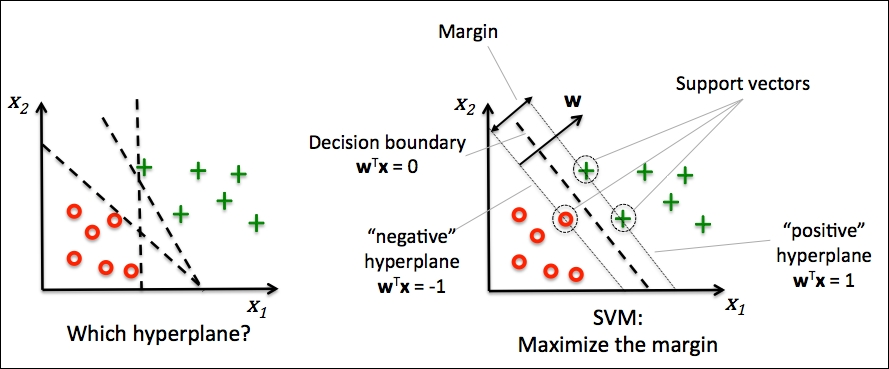
\includegraphics[width=.9\columnwidth]{svm_maximum_margin_support_vectors.jpg}%
\figcaption{\emph { Maximum Margin Classifier and Support Vectors in SVM}}}

\myfigure{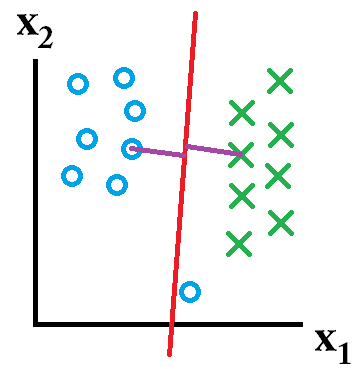
\includegraphics[width=0.3\columnwidth]{svm_outlier_cr.png}%
\figcaption{\emph { Outlier ignored in general SVM}}}


Only these \textbf{Support Vectors} contribute in finding the decision boundaries for the different categories, all other points/vectors don’t contribute anything to the model.

SVM looks at the very extreme case for finding the best boundaries, that is why SVM is very special and very different than most of the other Machine Learning models.

Note that the general SVM does not include \textbf{outliers} inside the decision boundary of its category.

But we can change the parameters of SVM to change the way a decision boundary is selected and can find the parameters which are best suited for our application.

\underline{Linearly Separable Dataset:}\\ \linebreak
Linearly Separable dataset can be easily classified using the above approach.

\underline{Non-Linearly Separable Dataset:}\\ \linebreak
For Non-Linearly Separable dataset, we cannot just simply separate the different categories using a simple line or hyperplane.

\begin{figure}[!h]
\begin{subfigure}[b]{.4\textwidth}
\centering
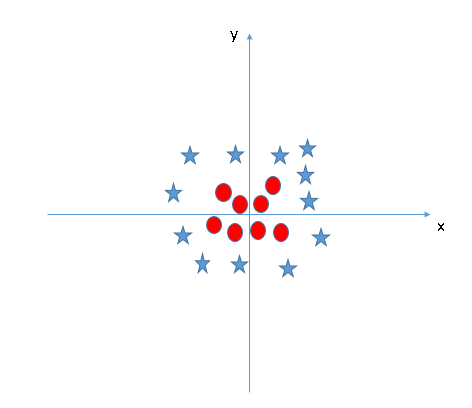
\includegraphics[width=7.5cm]{svm_non_linear.png}
\caption*{\centering \tiny Non-linearly separable data}
\end{subfigure}
\begin{subfigure}[b]{.5\textwidth}
\centering
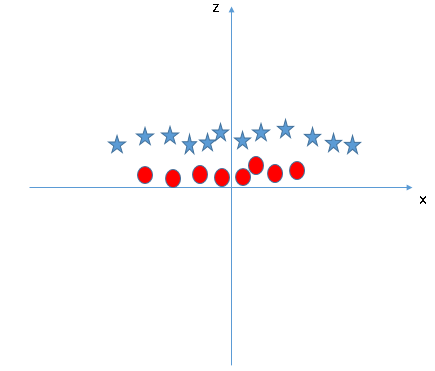
\includegraphics[width=6.7cm]{svm_non_linear_z_axis.png}
\caption*{\centering \tiny Mapping into higher dimension (adding z-axis\linebreak component) Z = \(x^2\) + \(y^2\)}
\end{subfigure}
\end{figure}


We are required to take our non-linearly separable dataset, map it to a higher dimension to make it linearly separable, build decision boundaries using SVM and then project all of that back into our original dimensions.

But calculating the transformations to a higher dimensional space can be highly compute intensive and might require a lot of computation and processing power.

So, to overcome this, we use a trick known as the \textbf{kernel trick}:

SVM does not need the actual vectors to work on it, it can do it only with the \textbf{dot products} between them. This dot product is called a \textbf{kernel function}.

This function will save us a lot of expensive calculations.

There are many kernel functions(kernels), some commonly used kernels are:
\begin{itemize}
\item Gaussian RBF kernel
\item Linear kernel
\item Sigmoid kernel
\item Polynomial kernel
\end{itemize}
\end{enumerate}
%\end{multicols}
\vspace{0.025\textheight} 
\myfigure{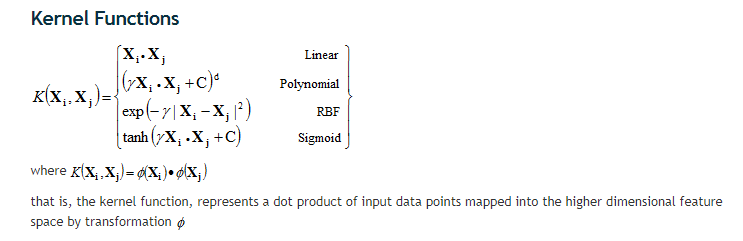
\includegraphics[width=0.9\columnwidth]{kernel_functions.png}%
\figcaption{\emph { Different Types of Kernel functions}}}
Sources:\linebreak
Fig 1: \url{https://www.packtpub.com/graphics/9781783555130/graphics/3547_03_07.jpg}\\ \linebreak
Fig 2: \url{https://stackoverflow.com/}\\ \linebreak
Fig 3: \url{https://www.analyticsvidhya.com/wp-content/uploads/2015/10/SVM_8.png}\\ \linebreak
Fig 4: \url{https://www.analyticsvidhya.com/wp-content/uploads/2015/10/SVM_9.png}\\ \linebreak
Fig 5: \url{http://www.statsoft.com/textbook/support-vector-machines} \\

\pagebreak
\section{\huge Studying SVM parameters \textbf{C} and \textbf{gamma}}
\begin{enumerate}
\item {\Large \textbf{The SVC penality parameter C :}} \\ 
\linebreak
\Large
In simple terms, a Support vector machine (for classification) mainly chooses a set of hyperplanes which classify the data into desired categories.
SVM finds the maximum margin hyperplanes using the nearest points of different categories.
However, perfect classification is present only in the ideal case, most of the time it is not possible to perfectly separate all points. 

In many cases we need to relax our maximum margin concept to classify most of the points correctly, these are known as soft margins. The role of penalty parameter of SVC class (sci-kit-learn python) becomes extremely important in such cases.

Low C value means our separating hyperplane is close to maximum margin hyperplane. Low C is helpful in ignoring the outliers. However, sometimes low C values give us poor accuracy, In our experiments, C = 1 gave as low as 53.61\% accuracy. Situations like these truly depend on the dataset, low C values provide room for diversity in a test set from a training set.In our case, it seems like data is under-fitted.

High C value means our separating hyperplane is at some distance from maximum margin hyperplane. High C value provides great fitting on the training set. However, sometimes higher C values may lead to overfitting, In our experiments, it was found that increasing C value drastically increases accuracy and then it slowly reduces on any further increment. Observations made are a clear indication that higher C value leads to overfitting the training data.\\
\counterwithin{figure}{section}
\begin{figure}[!h]
\centering
\begin{subfigure}[b]{0.3\textwidth}
  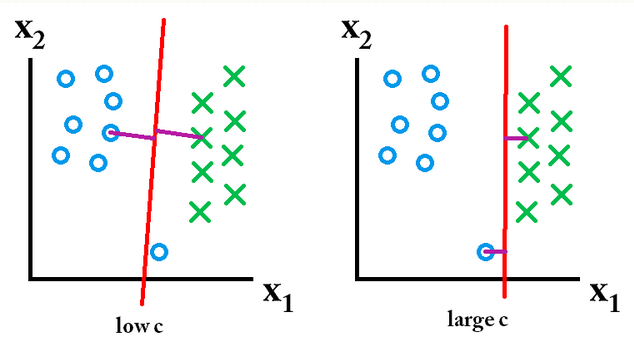
\includegraphics[width=\linewidth]{before.png}
  \caption{Training}
  \label{Fig:2}
\end{subfigure}
\begin{subfigure}[b]{0.3\textwidth}
  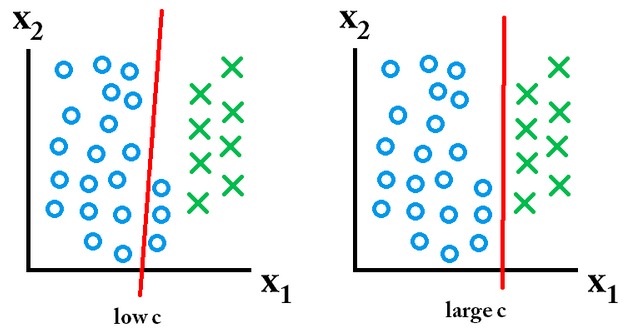
\includegraphics[width=\linewidth]{after.png}
  \caption{After testing}
  \label{Fig:2}
\end{subfigure}
\caption{low C and high C}
\emph{\normalsize Source: \url{https://stackoverflow.com/}\\}
\end{figure}
We changed values of the penalty parameter C and gamma (argument of an rbf kernel function) to observe the accuracy.
It was observed that C values close to 1000 in case of an rbf kernel and 10-100 in case of a linear kernel. Note that these observations were only on a specific test data (generated randomly).
Since, a relationship between the value of parameter C and Accuracy is highly dependent on the test set, we conducted More experiments (on many random test-train splits of our data) to determine the average accuracy of our model which will be discussed in subsequent sections of this project report.

\item \textbf{Importance of Gamma in case of non linear kernels:}\\
\linebreak
Gamma parameter is important only in case of non-linear kernels. A Linear kernel is independent of the value of Gamma. We have verified this point by doing experiments and can be seen in our plots for a linear kernel.Intuitively, high gamma makes the separator more non-linear and is better suited for a case when training data is nonlinearly separable.

Gamma parameter determines the role of a single support vector in determining the category of a point.
High gamma value means a support vector's center of influence is small and low gamma values imply big center of influence.
\begin{figure}[!h]
\centering
\begin{subfigure}[]{0.3\textwidth}
  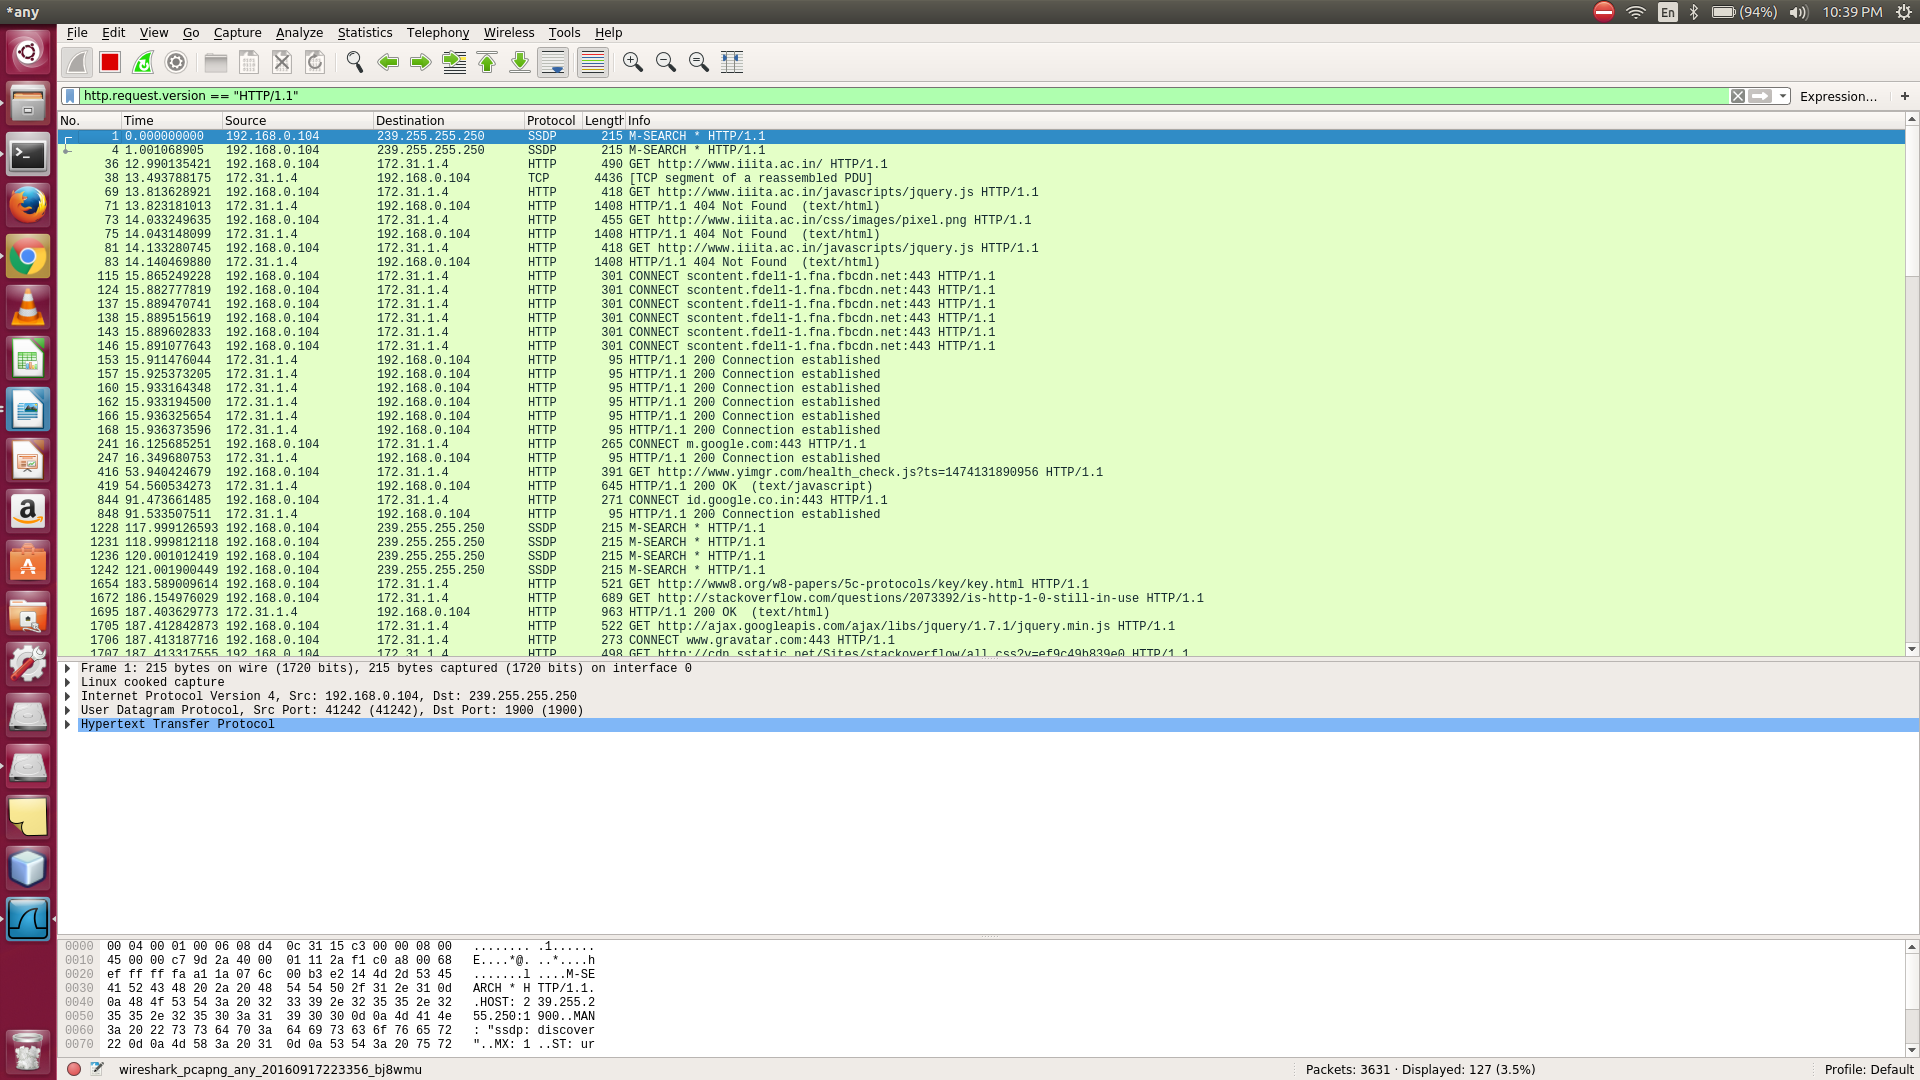
\includegraphics[width=\linewidth]{1.png}
  \caption{gamma= \(10^{-1} \) , C=\(10^{-2} \)}
  \label{Fig:2}
\end{subfigure}
\begin{subfigure}[]{0.3\textwidth}
  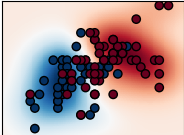
\includegraphics[width=\linewidth]{2.png}
  \caption{gamma= \(10^{0} \) , C=\(10^{-2} \)}
  \label{Fig:2}
\end{subfigure}
\begin{subfigure}[]{0.3\textwidth}
  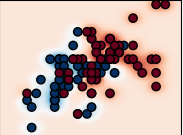
\includegraphics[width=\linewidth]{3.png}
  \caption{gamma= \(10^{1} \) , C=\(10^{-2} \)}
  \label{Fig:2}
\end{subfigure}

\begin{subfigure}[]{0.3\textwidth}
  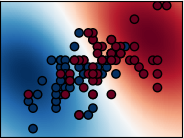
\includegraphics[width=\linewidth]{4.png}
  \caption{gamma= \(10^{-1} \) , C=\(10^{0} \)}
  \label{Fig:2}
\end{subfigure}
\begin{subfigure}[]{0.3\textwidth}
  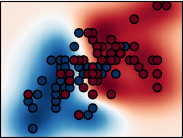
\includegraphics[width=\linewidth]{5.png}
  \caption{gamma= \(10^{0} \) , C=\(10^{0} \)}
  \label{Fig:2}
\end{subfigure}
\begin{subfigure}[]{0.3\textwidth}
  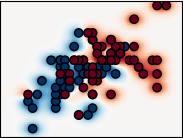
\includegraphics[width=\linewidth]{6.png}
  \caption{gamma= \(10^{1} \) , C=\(10^{0} \)}
  \label{Fig:2}
\end{subfigure}
\begin{subfigure}[]{0.3\textwidth}
  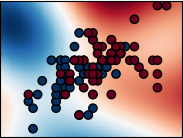
\includegraphics[width=\linewidth]{7.png}
  \caption{gamma= \(10^{-1} \) , C=\(10^{2} \)}
  \label{Fig:2}
\end{subfigure}
\begin{subfigure}[]{0.3\textwidth}
  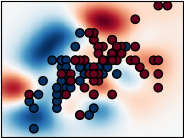
\includegraphics[width=\linewidth]{8.png}
  \caption{gamma= \(10^{0} \) , C=\(10^{2} \)}
  \label{Fig:2}
\end{subfigure}
\begin{subfigure}[]{0.3\textwidth}
  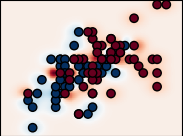
\includegraphics[width=\linewidth]{9.png}
  \caption{gamma= \(10^{1} \) , C=\(10^{2} \)}
  \label{Fig:2}
\end{subfigure}
\caption{ Gamma and C}
\emph{\normalsize Source : Sci-kit learn documentation}
\end{figure}
\end{enumerate}
\Large
\pagebreak
Quoting Scikit-learn documentation - " \emph{The gamma parameters can be seen as the inverse of the radius of influence of samples selected by the model as support vectors}"
\linebreak
 
It is observed that when gamma is very high the center of influence is diminished to the support vector itself.No value of C can be found which will reduce the overfitting of this model.If the test set has different characteristics than the training set then this model produces very bad accuracy.
On the other hand, if a value of gamma is chosen to be low, model fails to capture the unique details of data in case of non-linear kernels.\\ \linebreak
\linebreak
\textbf{C and Gamma}\\
\linebreak
From the above findings, it is clear the value of C and Gamma depends on our dataset.

The image below from sci-kit learn documentation depicts the combined effect of C and Gamma on a simple classification problem.\\
\pagebreak
\pagebreak
%---------------------------------------------------------------------------
\pagebreak
\counterwithin{figure}{section}
\section{\Huge Methodology Flow Diagram}
\begin{figure}[!h]
  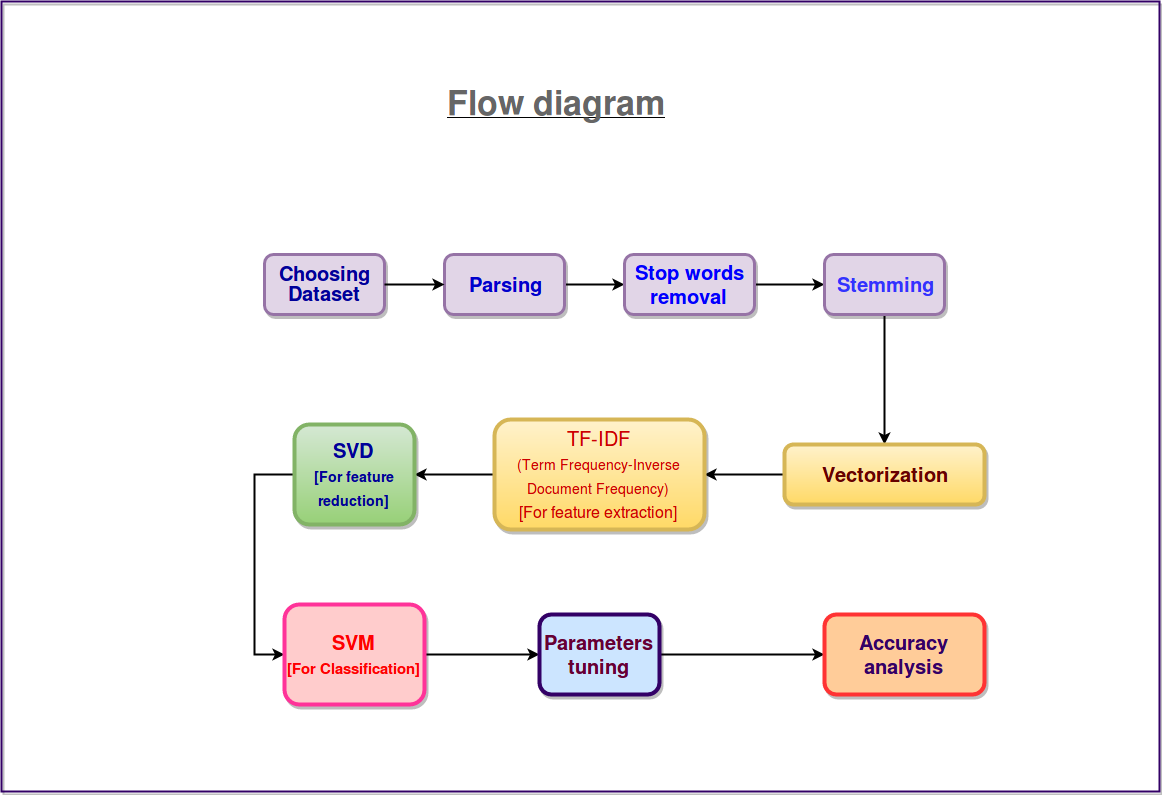
\includegraphics[width=\linewidth]{Flowchart.png}
  \caption{Flow diagram}
  \label{Fig:2}
\end{figure}
\pagebreak
%----------------------------------------------------------------------------------------
\section{\Huge Literature survey}
\counterwithin{table}{section}
\begin{table}[!h]
\raggedleft
\label{Fig:}
\begin{tabular}{|p{0.6cm}|p{2.5cm}|p{0.6cm}|p{3.3cm}|p{5.1cm}|p{2.0cm}|}
\hline
\textbf{S.no.} & \textbf{Paper Title}                                                           & \textbf{Year} & \textbf{Journal/Conference}                                                                                   & \textbf{Abstract}                                                                                                                                                                                                                                                                                                                                                   & \textbf{Author}                                       \\ \hline
1.\rule{0pt}{3ex}              & Inductive learning algorithms and representations for text categorization \cite{Dumais:1998:ILA:288627.288651}       & 1998          & 7th International Conference on Information and knowledge management1998-11-01                                & In this paper five different  algorithms for text classification have been compared like find similar, decision trees, naive bayes,bayes nets and SVM.The best result were found using SVM . So it guided us to choose SVM for classification.                                                                                                                      & Susan Dumais,Mehran Sahami,John Platt,David Heckerman \\ \hline
2\rule{0pt}{3ex}             & A Statistical Learning Model of Text Classification forSupport Vector Machines \cite{Joachims:2001:SLL:383952.383974} & 2001          & 24th annual international ACM SIGIR conference on Research and development in information retrieval2001-09-01 & In this paper the statistical properties of text-classification tasks is conneccted with generalizaton performance of SVM. It explained why and when SVMs perform well for text classification.                                                                                                                                                                     & Thorsten Joachims                                     \\ \hline
3.\rule{0pt}{3ex}              & High-performing feature selection for text classification \cite{Rogati:2002:HFS:584792.584911}                      & 2002          & 11th International Conference on Information and knowledge management2002-11-04                               & This paper mainly focuses on the importance of feature selection and feature reduction in text classification. Here various techniques have been discussed on different machine learning algorithms for feature reduction.In this paper CHI\_MAX and IG methods have been combined for giving weights. For reducing redundancy \(\mu\) co-occurence method is used here. & Monica Rogati,Yiming Yang                             \\ \hline
4.\rule{0pt}{3ex}              & Transductive Inference for Text Classification using Support Vector Machines \cite{joachims1999transductive}   & 1999          & 16th International Conference on Machine Learning27-06-1999                                                   & In this paper the concept of Transductive SVM (TSVM)  is introduced. It explains us the limitations of normal SVM in some cases where TSVM are better than SVM. The experiments here tells us about significant improvement of TSVM over inductive methods. TSVMs work very well in cases where there is smaller training dataset than the test set.                & Thorsten Joachims                                     \\ \hline
5.\rule{0pt}{3ex}              & An Optimal SVM-Based Text Classification Algorithm \cite{wang2006optimal}                             & 2006          & International Conference on Machine Learning and Cybernetics13/09/2006                                        & This paper describes new algorithms for feature selection which highly optimize the efficiency of classification. The new algorithm applies entropy weighing scheme for feature selection in a newer way. Also optimal parameter settings have been used to get better results.                                                                                     & Zi-Qiang Wang, Xia Sun, De-Xian Zhang, Xin Li         \\ \hline
\end{tabular}
\caption{Literature survey}
\end{table}
\pagebreak
%----------------------------------------------------------------------------------------

%----------------------------------------------------------------------------------------
\section{\Huge Experiments}
\hspace*{-1cm}
\begin{table}[!h]
\centering
\begin{tabular}{|p{0.7cm}|p{4.1cm}|p{2.4cm}|p{2cm}|p{2.5cm}|p{2.5cm}|}
\hline
\textbf{S.No.} & \textbf{Kernel}             & \textbf{Penalty \t Parameter (C)} & \textbf{Kernel \linebreak Coefficient (gamma)} & \textbf{Training Time (in seconds)} & \textbf{Accuracy \linebreak (\% age)} \\ \hline
1.1            & Radial Basis Function (rbf) & 1                               & 0                                   & 14.7179185738                       & 53.5163776493              \\ \hline
1.2            & Radial Basis Function (rbf) & 1                               & 5                                   & 20.2596582446                       & 88.2947976879              \\ \hline
1.3            & Radial Basis Function (rbf) & 1                               & 10                                  & 49.7798475756                       & 86.8015414258              \\ \hline
2.1            & Radial Basis Function (rbf) & 10                              & 0                                   & 10.9192837309                       & 80.9730250482              \\ \hline
2.2            & Radial Basis Function (rbf) & 10                              & 5                                   & 19.5810598891                       & 88.9691714836              \\ \hline
2.3            & Radial Basis Function (rbf) & 10                              & 10                                  & 50.6595395278                       & 87.2350674374              \\ \hline
3.1            & Radial Basis Function (rbf) & 100                             & 0                                   & 7.2436635578                        & 86.7052023121              \\ \hline
3.2            & Radial Basis Function (rbf) & 100                             & 5                                   & 19.2433398237                       & 88.2947976879              \\ \hline
3.3            & Radial Basis Function (rbf) & 100                             & 10                                  & 50.6608579851                       & 87.1868978805              \\ \hline
4.1            & Radial Basis Function (rbf) & 1000                            & 0                                   & 6.0687723209                        & 88.1502890173              \\ \hline
4.2            & Radial Basis Function (rbf) & 1000                            & 5                                   & 19.1799743322                       & 88.2947976879              \\ \hline
4.3            & Radial Basis Function (rbf) & 1000                            & 10                                  & 50.5428827899                       & 87.1868978805              \\ \hline
5.1            & Radial Basis Function (rbf) & 10000                           & 0                                   & 6.2777937673                        & 87.6685934489              \\ \hline
5.2            & Radial Basis Function (rbf) & 10000                           & 5                                   & 19.1768832492                       & 88.2947976879              \\ \hline
5.3            & Radial Basis Function (rbf) & 10000                           & 10                                  & 50.9507252798                       & 87.1868978805              \\ \hline
6.1            & Radial Basis Function (rbf) & 100000                          & 0                                   & 7.1739251665                        & 87.5722543353              \\ \hline
6.2            & Radial Basis Function (rbf) & 100000                          & 5                                   & 19.1878773779                       & 88.2947976879              \\ \hline
6.3            & Radial Basis Function (rbf) & 100000                          & 10                                  & 50.5921981372                       & 87.1868978805              \\ \hline
7.1            & Radial Basis Function (rbf) & 1000000                         & 0                                   & 9.7328505405                        & 87.1868978805              \\ \hline
7.2            & Radial Basis Function (rbf) & 1000000                         & 5                                   & 19.2118927153                       & 88.2947976879              \\ \hline
7.3            & Radial Basis Function (rbf) & 1000000                         & 10                                  & 50.5413184316                       & 87.1868978805              \\ \hline
\end{tabular}
\caption{Change in \textbf{Accuracy} and \textbf{Training time} with change in SVC parameter \textbf{C} and \textbf{gamma} [for \textbf{‘rbf’} kernel]}
\label{my-table}
\end{table}\hspace*{-1cm}
\hspace*{-4cm}
\vspace*{2cm}
\begin{table}[!h]
\centering
\begin{tabular}{|p{0.7cm}|p{4.1cm}|p{2.4cm}|p{2cm}|p{2.5cm}|p{2.5cm}|}
\hline
\textbf{S.No.} & \textbf{Kernel} & \textbf{Penalty\linebreak Parameter\linebreak (C)} & \textbf{Training Time (in seconds)} & \textbf{Accuracy \linebreak(\% age)} \\ \hline
1              & Linear          & 1                                & 5.7447666912                        & 85.5973025048              \\ \hline
2              & Linear          & 10                               & 4.4802451655                        & 88.4393063584              \\ \hline
3              & Linear          & 100                              & 4.4675985817                        & 87.9094412331              \\ \hline
4              & Linear          & 1000                             & 5.3948755933                        & 87.4759152216              \\ \hline
5              & Linear          & 10000                            & 10.4627913232                       & 87.1868978805              \\ \hline
6              & Linear          & 100000                           & 101.2622459789                      & 87.0905587669              \\ \hline
\end{tabular}
\caption{Change in \textbf{Accuracy} and \textbf{Training time} with change in SVC parameter \textbf{C}  [for \textbf{‘linear’} kernel]}
\label{my-table}
\end{table}
\pagebreak
%\begin{multicols}{2}
\subsection{\LARGE Observations :}
Using different values for the \textbf{Penalty Parameter (C)} and \textbf{Kernel coefficient (gamma)}, we found that:\\
\linebreak
\linebreak
{For \textbf{‘rbf’} kernel:}
\setlength{\itemsep}{0cm}
\begin{itemize}
\item For a fixed \textbf{gamma} value,with the increase in the value of \textbf{C}, the accuracy of our predictions increased gradually, reached a certain maximum value and then decreased gradually or remained constant. This observation can be justified because as we increase the value of \textbf{C}, the generality of the classification model is also decreased and is somewhat lost with very large value of \textbf{C} as the model tries to include every outlier inside the correct decision boundary and results in overfitting the training data.

\end{itemize}
For \textbf{‘linear’} kernel:
\begin{itemize}
\item Training time increased with increasing value of \textbf{C}, and increases by a high amount after \textbf{C = 10000}.
\item \textbf{gamma} parameter have NO significance for the \textbf{‘linear’} kernel function.
\end{itemize}
\subsection{\LARGE Best results :}
The following are the best results we found from our experiments:\\
\linebreak
For \textbf{‘rbf’} kernel:
\begin{itemize}
\item C = 10.0
\item gamma = 5.0
\item Training Time taken = 19.581059889092217 seconds
\item Accuracy on test dataset = 88.969171483622356 \%
\end{itemize}
For \textbf{‘linear’} kernel:
\begin{itemize}
\item C = 10.0 
\item Training Time taken = 4.48024516547855 seconds
\item Accuracy on test dataset = 88.439306358381498 \%
\end{itemize}
After taking these observations, we then took the values of the svc parameters C and gamma of the 5 most accurate observations.
We then used these 5 most accurate observations to computed the Average Accuracy and Average Training time with different 
random splits of training and test, for both the ‘rbf’ and the ‘linear’ kernel.
%\end{multicols}
\pagebreak
\subsection{\LARGE Use of random training and test dataset:}
\begin{table}[!h]
\centering
\begin{tabular}{|p{0.7cm}|p{1.5cm}|p{1.8cm}|p{1.9cm}|p{2.3cm}|p{2.3cm}|p{2.3cm}|p{2.3cm}|}
\hline
\textbf{S.No.} & \textbf{Kernel}             & \textbf{Penalty Parameter (C)} & \textbf{Kernel Coefficient (gamma)} & \textbf{Average Training \linebreak Time \linebreak (in seconds)} & \textbf{Average \linebreak Accuracy \linebreak (\% age)} & \textbf{Minimum \linebreak Accuracy \linebreak (\% age)} & \textbf{Maximum \linebreak Accuracy \linebreak (\% age)} \\ \hline
1              & Radial Basis Function (rbf) & 10                              & 5                                   & 19.5975905119                               & 87.591522158                       & 86.8497109827                     & 88.1984585742                     \\ \hline
2              & Radial Basis Function (rbf) & 1                               & 5                                   & 19.8280292122                               & 88.2369942197                      & 88.0539499037                     & 88.3429672447                     \\ \hline
3              & Radial Basis Function (rbf) & 100                             & 5                                   & 19.1036437403                               & 86.5317919075                      & 85.9344894027                     & 86.7052023121                     \\ \hline
4              & Radial Basis Function (rbf) & 1000                            & 5                                   & 18.7571186214                               & 87.9768786127                      & 87.1868978805                     & 88.1984585742                     \\ \hline
5              & Radial Basis Function (rbf) & 10000                           & 5                                   & 20.2823468282                               & 88.7379576108                      & 87.8612716763                     & 89.2581888247                     \\ \hline
\end{tabular}
\caption{Computation of \textbf{Average Accuracy} and \textbf{Average Training time} with different random splits of training and test data for fixed value of SVC parameters \textbf{C} and \textbf{gamma} [for \textbf{‘rbf’} kernel]}
\label{my-table}
\end{table}


\begin{table}[!h]
\centering
\begin{tabular}{|p{0.7cm}|p{1.5cm}|p{2.3cm}|p{2.3cm}|p{2.3cm}|p{2.3cm}|p{2.3cm}|p{2.3cm}|}
\hline
\textbf{S.No.} & \textbf{Kernel} & \textbf{Penalty\linebreak Parameter\linebreak (C)} & \textbf{Average Training\linebreak Time\linebreak(in seconds)} & \textbf{Average Accuracy\linebreak (\% age)} & \textbf{Minimum Accuracy\linebreak (\% age)} & \textbf{Maximum Accuracy \linebreak (\% age)} \\ \hline
1              & Linear          & 10                              & 26.4541190135                               & 86.3102119461                      & 85.3082851638                     & 87.6685934489                     \\ \hline
2              & Linear          & 100                             & 19.0949781875                               & 87.3603082852                      & 86.6570327553                     & 88.8728323699                     \\ \hline
3              & Linear          & 1000                            & 26.5995590032                               & 85.4624277457                      & 84.4894026975                     & 86.8978805395                     \\ \hline
4              & Linear          & 10000                           & 19.1290173923                               & 87.2832369942                      & 86.4161849711                     & 88.5356454721                     \\ \hline
5              & Linear          & 100000                          & 22.8623470763                               & 88.1695568401                      & 87.4759152216                     & 89.0655105973                     \\ \hline
\end{tabular}
\caption{Computation of \textbf{Average Accuracy} and \textbf{Average Training time} with different random splits of training and test data for fixed value of SVC parameter \textbf{C} [for \textbf{‘linear kernel'}]}
\label{my-table}
\end{table}
\pagebreak
%\begin{multicols}{2}
\subsection{\LARGE Observations :}
Using different random splits of training and test datasets for fixed value of svc parameters, we found that:\\
\linebreak
\linebreak
For \textbf{‘rbf’} kernel:
\begin{itemize}
\item All the top 5 most accurate observations were found having gamma = 5.0 .
\item We found that the best result found on average basis is having different \textbf{C} parameter from the best result found previously. This is the result of the change in training and test dataset, which shows that the accuracy depends heavily on the training data, as well as the test data on which the model is to be tested of the same dataset. So, we cannot fix the value of the parameters \textbf{C} and \textbf{gamma} 
and say that these are the perfect parameter values for this dataset. The parameter values which are best for a specific split of training and test data may not be the best for any other split.
\item So, we cannot find the perfect parameter values for the dataset if the training and test datasets are applicable to  changes but we can find the perfect parameter values for a dataset with fixed training and test dataset.
\item We even reached 89.25 \% accuracy for some random splitting of out dataset in our last observation, which also turned out to be the best observation.
\end{itemize}
For \textbf{‘linear’} kernel:
\begin{itemize}
\item In this case also we have different best results for the same reason as above.
\item Here also we reached 89.06 \% accuracy for some random splitting of out dataset in our last observation, which also turned out to be the best observation.
\end{itemize}
\subsection{\LARGE Best results :}

The following are the best results we found from our experiments:
For \textbf{‘rbf’} kernel:
\begin{itemize}
\item C = 10000.0
\item gamma = 5.0
\item Average Training Time taken = 20.28234682823986 seconds
\item Average Accuracy on test dataset = 88.737957610789986 \%
\end{itemize}
For \textbf{‘linear’} kernel:
\begin{itemize}
\item C = 100000.0
\item Average Training Time taken = 22.862347076279367 seconds
\item Average Accuracy on test dataset = 88.169556840077068 \%
\end{itemize}
%\end{multicols}
\pagebreak
%----------------------------------------------------------------------------------------
\subsection{\textbf \Large {Accuracy }vs\textbf{ Penalty Parameter (C) graphs :-}}
\subsubsection{\textbf \Large  {For linear kernel :}}
\begin{figure}[!h]
  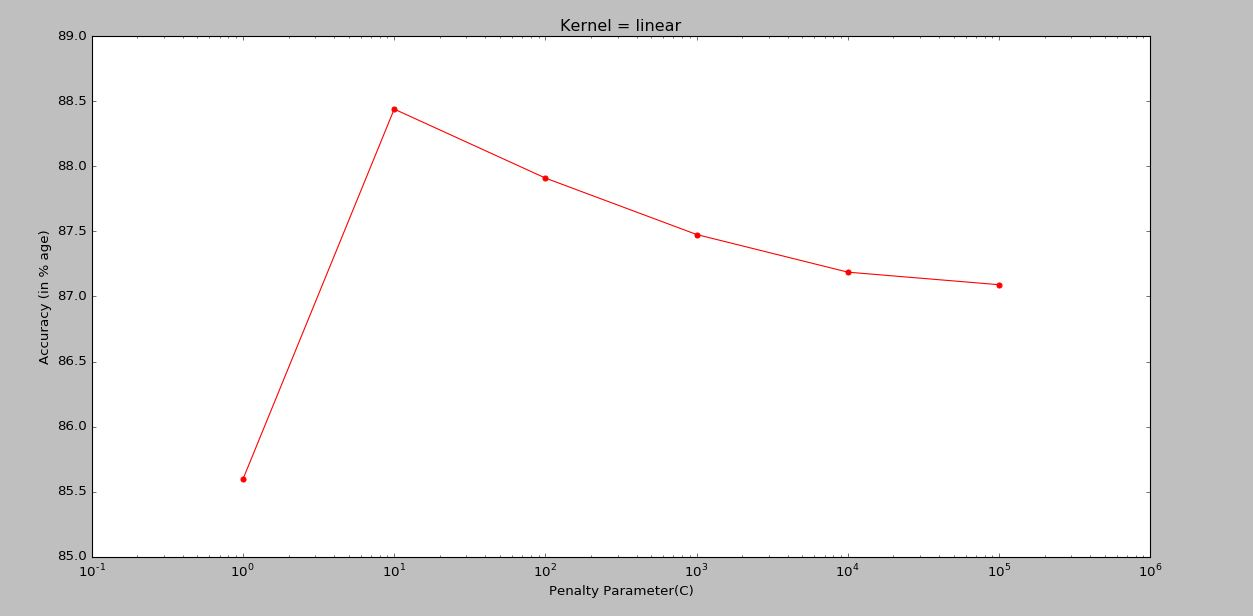
\includegraphics[width=\linewidth]{linear.JPG}
  \caption{\textbf{Accuracy }vs\textbf{ Penalty Parameter (C)} (for \textbf{linear kernel})}
  \label{fig:}
\emph{\normalsize Standard deviation = 0.964835}
\end{figure}

\begin{figure}[!h]
  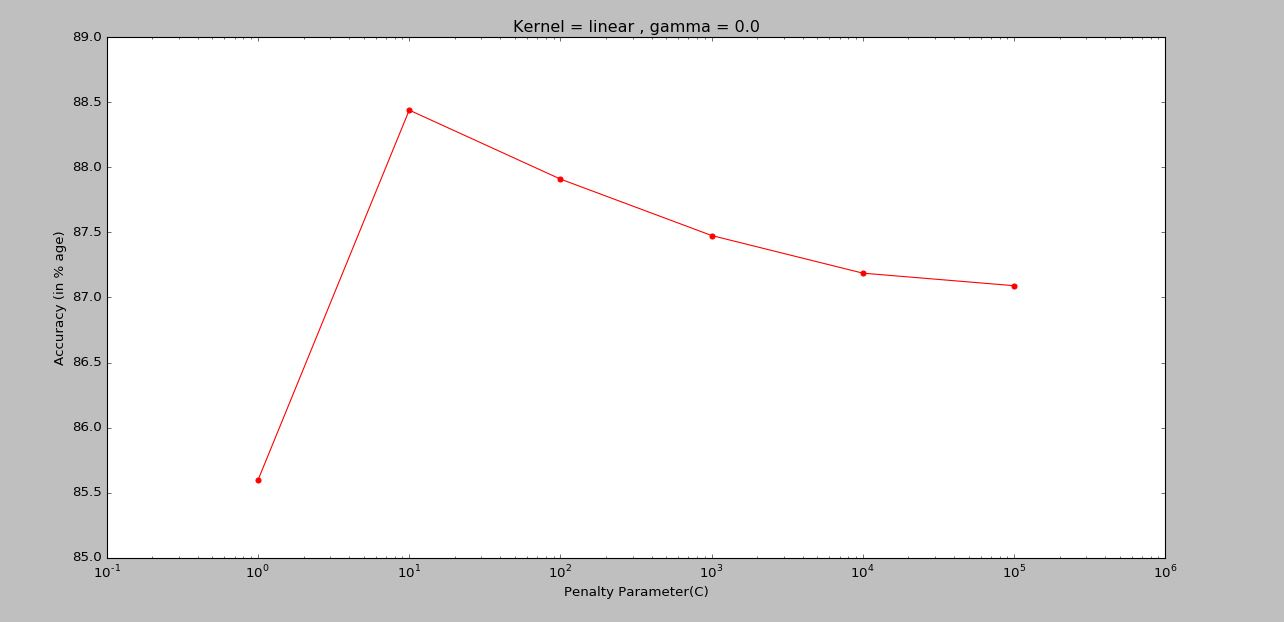
\includegraphics[width=\linewidth]{linear_1.JPG}
  \caption{\textbf{Accuracy }vs\textbf{ Penalty Parameter (C)} (for \textbf{linear kernel} with \textbf{gamma} = 0.0)}
  \label{fig:}
  \emph{\normalsize Standard deviation = 0.964835}
\end{figure}

\pagebreak
\begin{figure}[!h]
  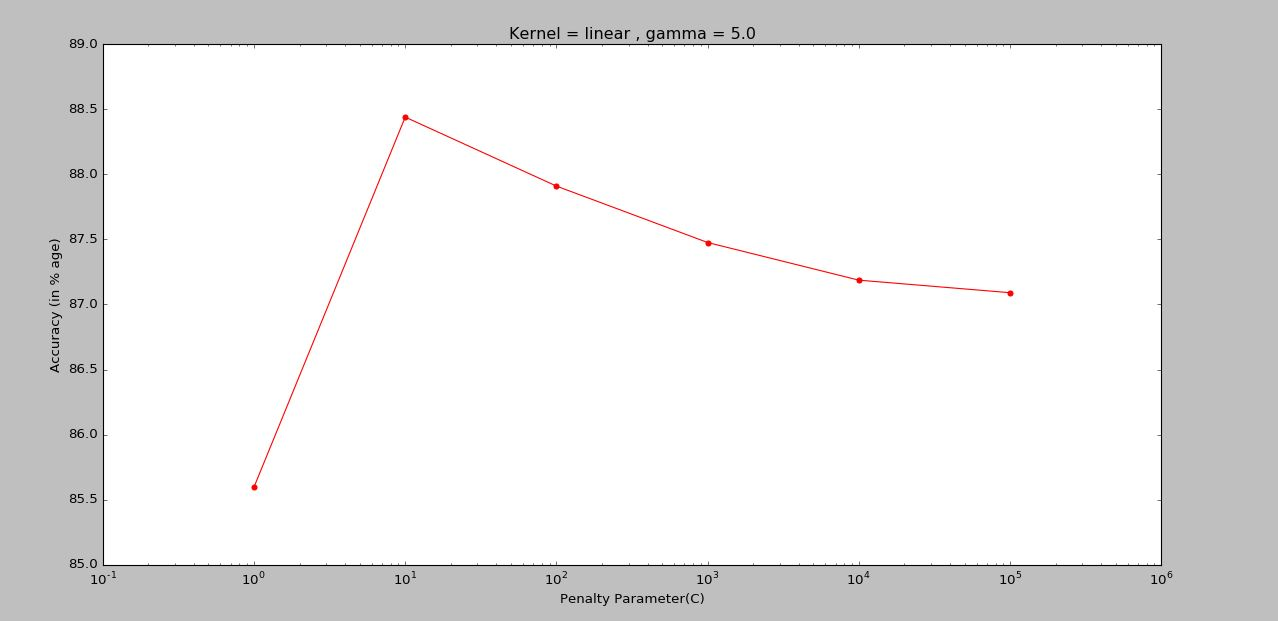
\includegraphics[width=\linewidth]{linear_2.JPG}
  \caption{\textbf{Accuracy }vs\textbf{ Penalty Parameter (C)} (for \textbf{linear kernel} with \textbf{gamma} = 5.0)}
  \label{fig:}
  \emph{\normalsize Standard deviation = 0.964835}
\end{figure}

\begin{figure}[!h]
  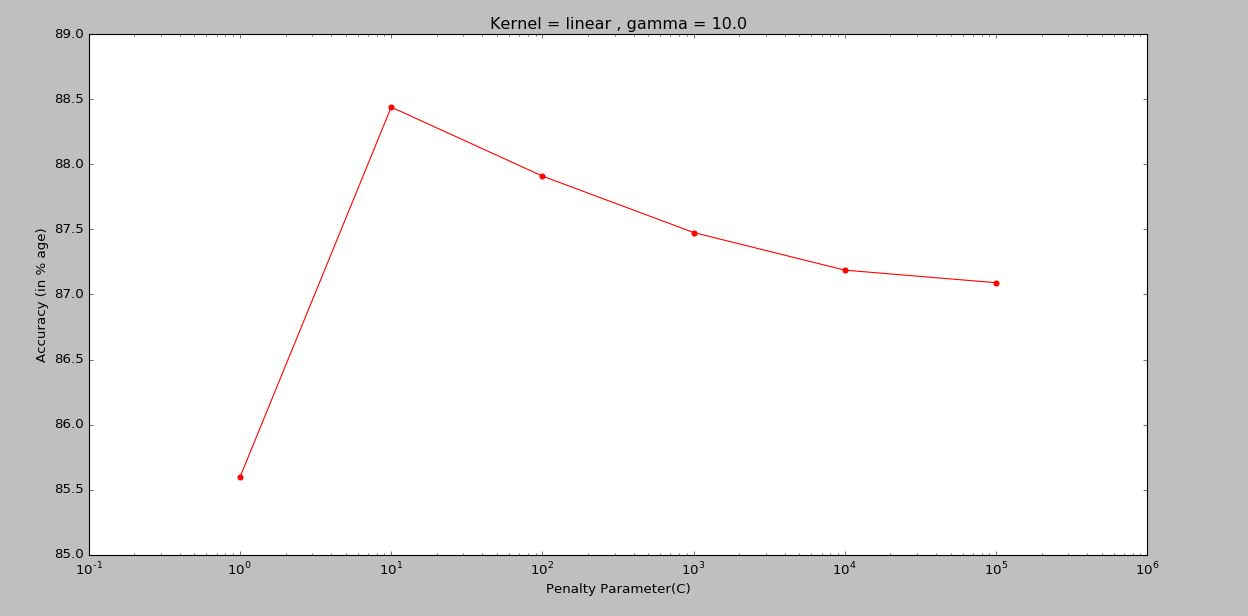
\includegraphics[width=\linewidth]{linear_3.JPG}
  \caption{\textbf{Accuracy }vs\textbf{ Penalty Parameter (C)} (for \textbf{linear kernel} with \textbf{gamma} = 10.0)}
  \label{fig:}
  \emph{\normalsize Standard deviation = 0.964835}
\end{figure}

\pagebreak
\begin{figure}[!h]
  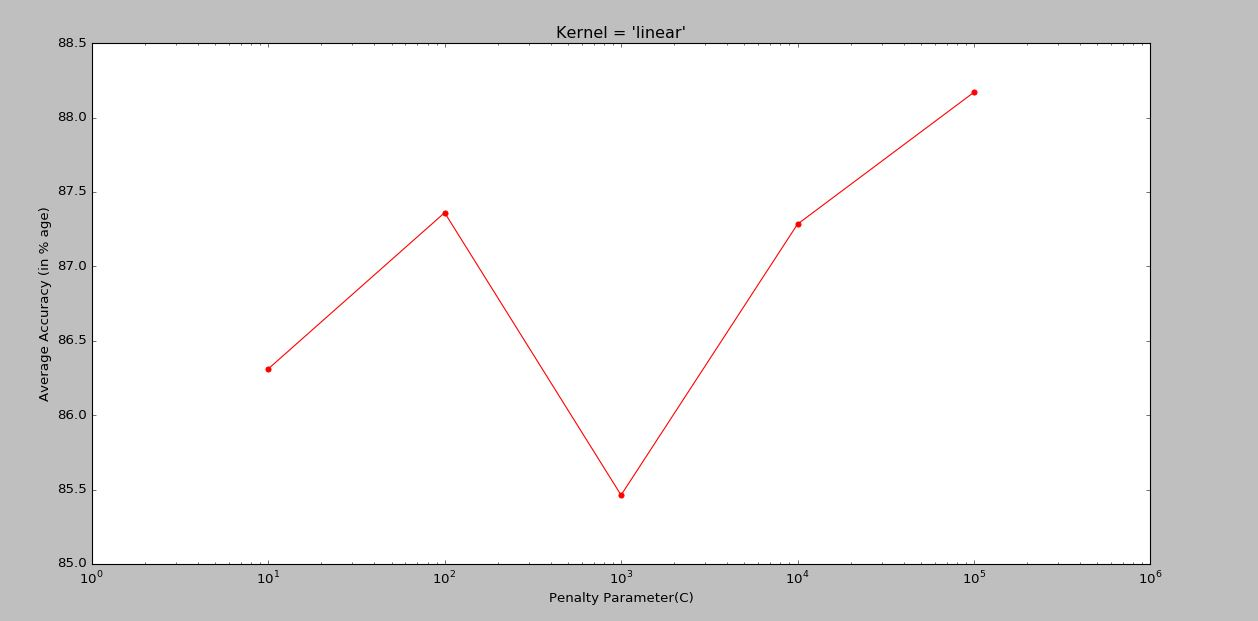
\includegraphics[width=\linewidth]{linear_for_different_randomstates.JPG}
  \caption{\textbf{Accuracy }vs\textbf{ Penalty Parameter (C)} (for \textbf{linear kernel} with different splits of training and test data)}
  \label{fig:}
  \emph{\normalsize Standard deviation = 1.046843}
\end{figure}

We can clearly see that the accuracy for the test data varies by a good amount for different splits of training and test data.\\
\linebreak
\ This shows that the accuracy depends heavily on the data on which the model is trained, as well as the future data on which it will be tested. 


\subsubsection{\textbf \Large  {For rbf kernel :}}
\begin{figure}[!h]
  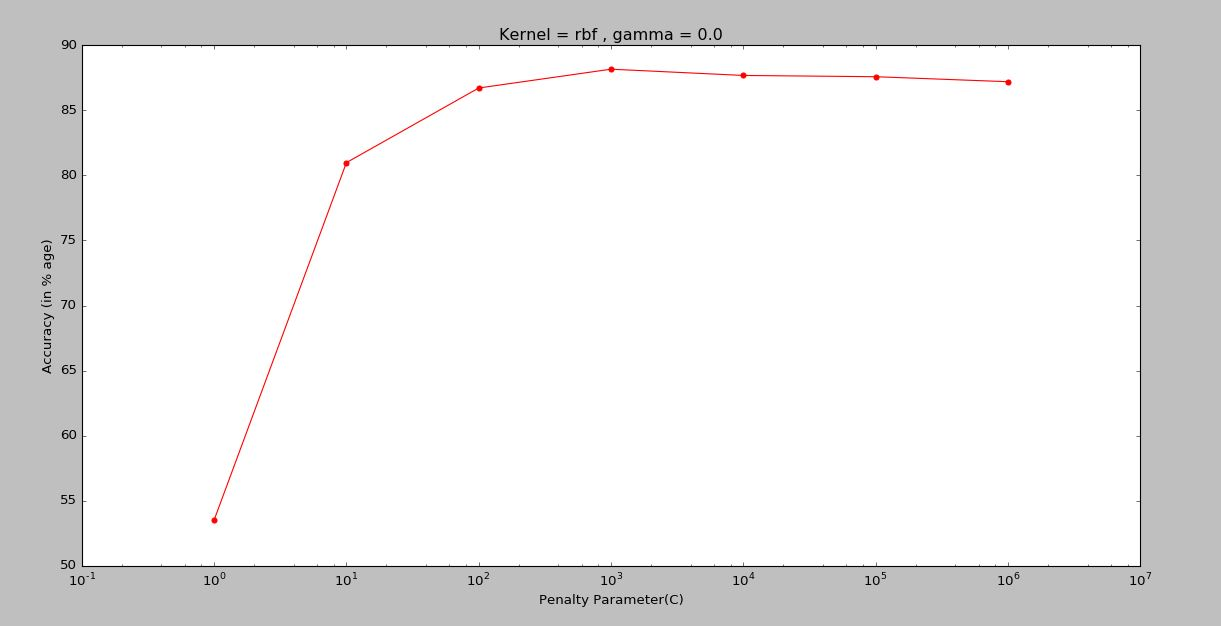
\includegraphics[width=\linewidth]{rbf_1.JPG}
  \caption{\textbf{Accuracy }vs\textbf{ Penalty Parameter (C)} (for \textbf{rbf kernel} with \textbf{gamma} = 0.0)}
  \label{fig:}
  \emph{\normalsize Standard deviation = 12.660401}
\end{figure}
\pagebreak
\begin{figure}[!h]
  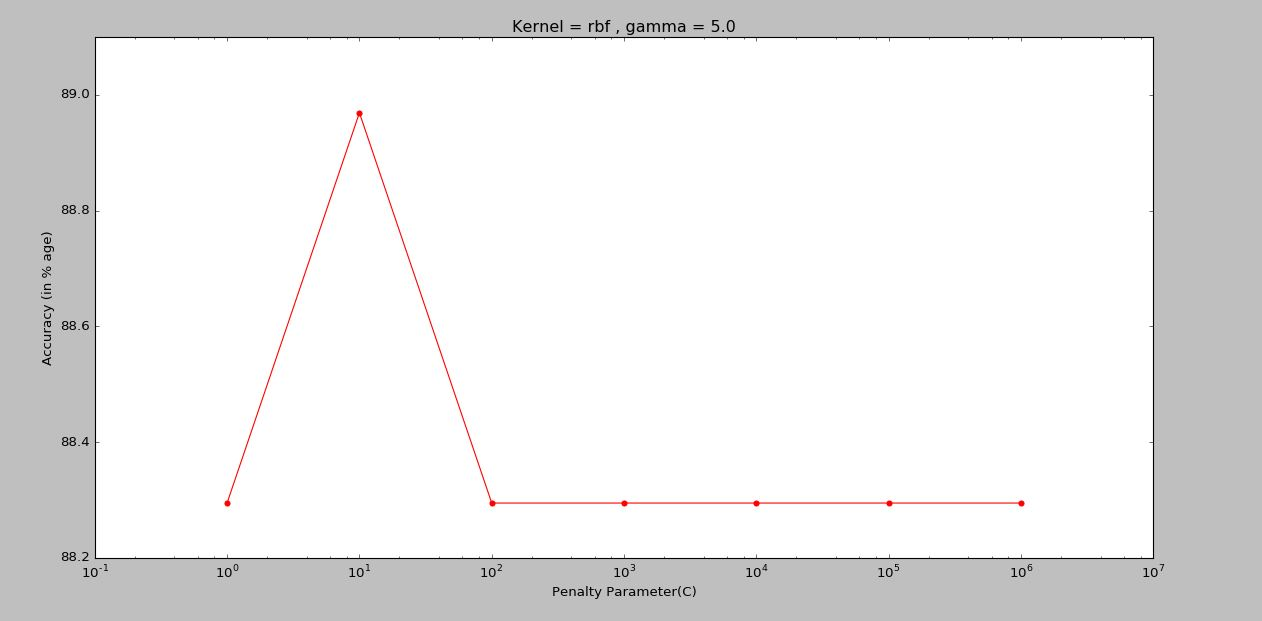
\includegraphics[width=\linewidth]{rbf_2.JPG}
  \caption{\textbf{Accuracy }vs\textbf{ Penalty Parameter (C)} (for \textbf{rbf kernel} with \textbf{gamma} = 5.0)}
  \label{fig:}
  \emph{\normalsize Standard deviation = 0.254889}
\end{figure}

\begin{figure}[!h]
  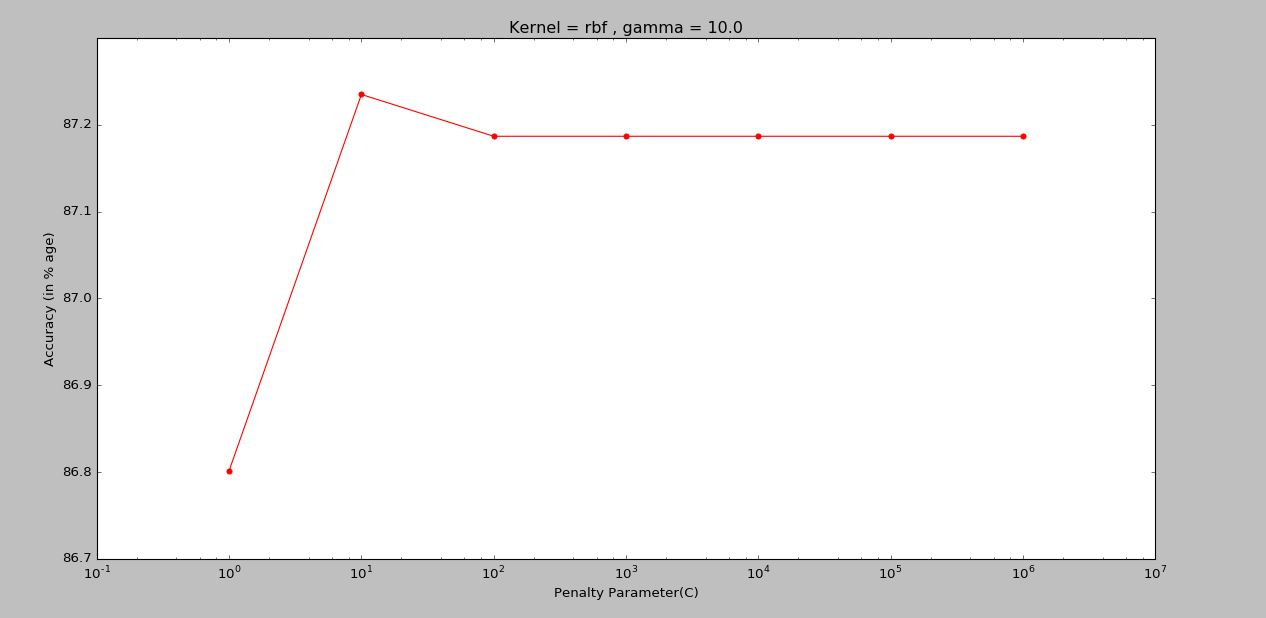
\includegraphics[width=\linewidth]{rbf_3.JPG}
  \caption{\textbf{Accuracy }vs\textbf{ Penalty Parameter (C)} (for \textbf{rbf kernel} with \textbf{gamma} = 10.0)}
  \label{fig:}
  \emph{\normalsize Standard deviation = 0.149765}
\end{figure}
\pagebreak
\begin{figure}[!h]
  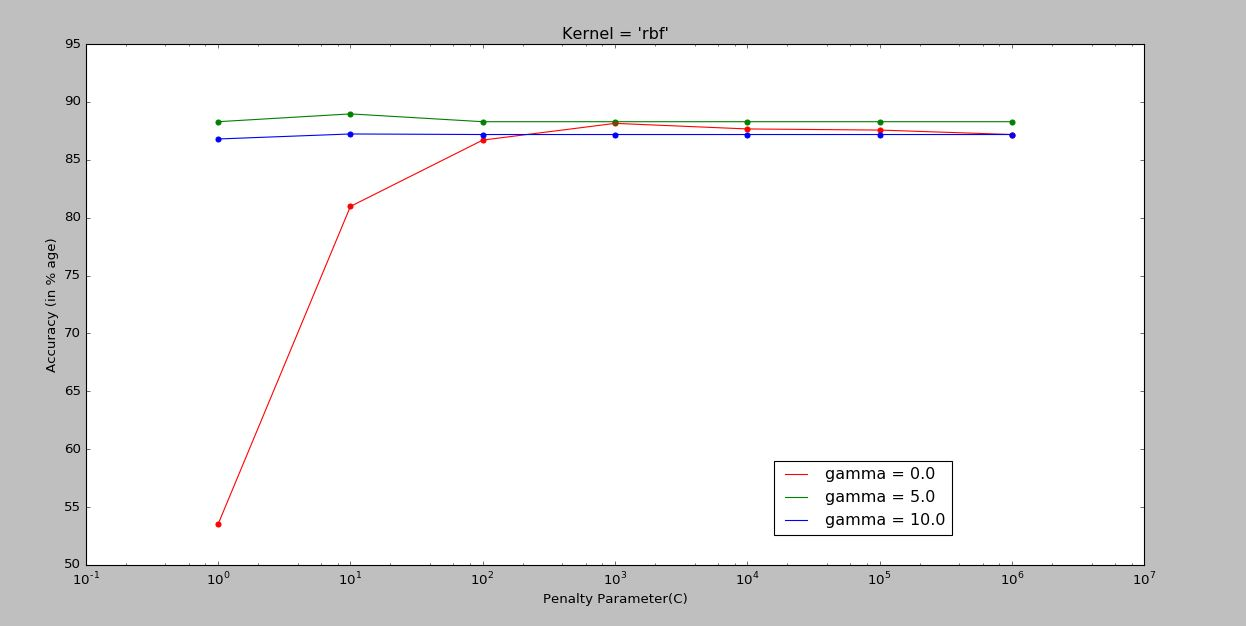
\includegraphics[width=\linewidth]{rbf_all_in_one.JPG}
  \caption{\textbf{Accuracy }vs\textbf{ Penalty Parameter (C)} (for \textbf{rbf kernel})}
  \label{fig:}
\end{figure}

\begin{figure}[!h]
  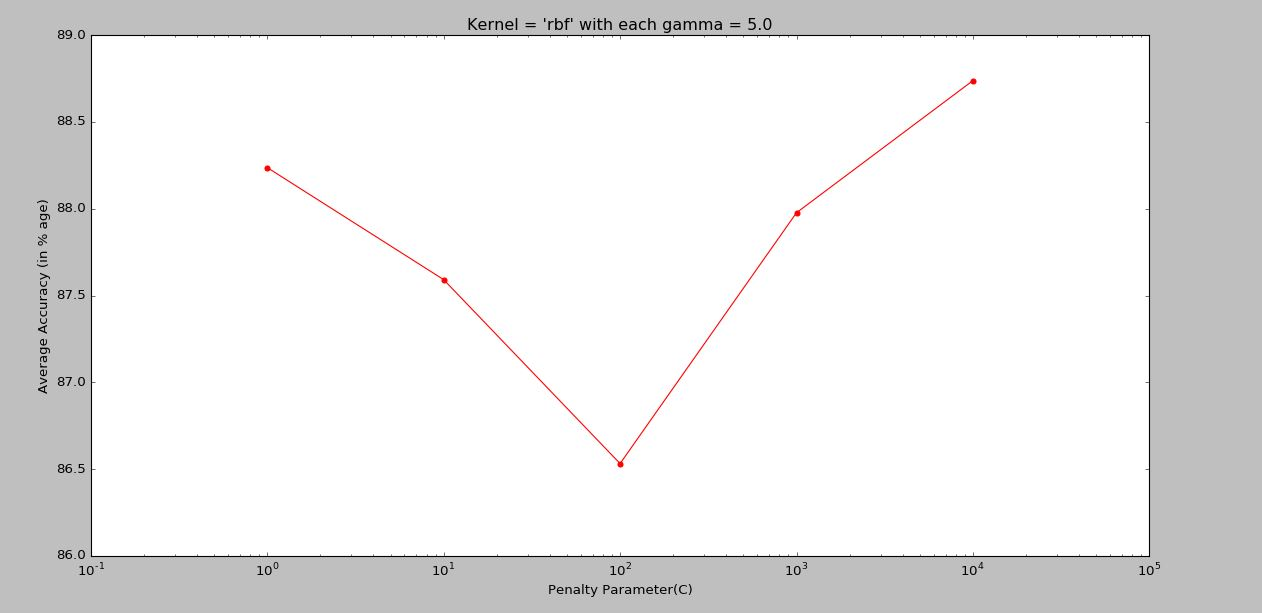
\includegraphics[width=\linewidth]{kuchbhi.jpg}
  \caption{\textbf{Accuracy }vs\textbf{ Penalty Parameter (C)} (for \textbf{rbf kernel} with different splits of training and test data)}
  \label{fig:}
  \emph{\normalsize Standard deviation = 0.829563}
\end{figure}

Here also we can clearly see that the accuracy for the test data varies by a good amount for different splits of training and test data.\\
\linebreak
\ \ This shows that the accuracy depends heavily on the data on which the model is trained, as well as the future data on which it will be tested. 
\pagebreak

\section{\Huge Generic Text Classifier}
\Large
After training, testing and analysing various parameter of SVM function on various kernels for getting the best accuracy results on "Reuters Dataset".

\begin{itemize}
\item We have created a generic text classification model which can be used on many datasets by applying minor changes in the code and sometimes without any changes.
\item We tested our text classification model on various small datasets like News headline classifier \cite{news_headline}, amazon reviews \cite{Lichman:2013}, IMDb movie reviews \cite{Lichman:2013}, Yelp reviews \cite{Lichman:2013} and SMS Spam Collection \cite{sms_spam} etc.

\item The tests we did was on the same dataset obtained by splitting datasets into training and testing parts
\end{itemize}
We did binary classification (positive or negative) on review datasets:-
\linebreak \linebreak
\textbf{\LARGE Results Obtained:}\\ \\
The average accuracy obtained for various datasets:-\\
\linebreak
\Large
1. Amazon review = 75.74\% ( data size = 1000 , kernel = linear )\\ \\
2. IMDb review = 73.83\% ( data size = 1000 , kernel = linear )\\ \\
3. Yelp review = 77.03\% ( data size = 1000 , kernel = linear )\\ \\
4. Spam Detection = 96.34\% ( best we obtained till now , data size = 5574 , kernel = linear )\\ \\
5. News Headline = 90.71\% ( data size = 5977 , kernel = rbf )\\ \\
All these were having 100 random states.
\pagebreak

\section*{\Huge Amazon Online Review Binary-Classifier}
\Large
For amazon review dataset we trained it and tested it on the splitted portion, 
Once this part was over, we modified our model and made it online ,

\begin{itemize}
\item now it takes review from user.
\item extracts and reduces the features complete dataset (original+user input) using SVD.
\item training is done only for our previous dataset.
\item then the review is accordingly classified
\item the user entered review is added to our dataset after classification
\end{itemize}

This added data helps us to improve accuracy if similar input is given again.\\ \\ \\ \\
\section {\Huge Future Work}
\Large
Till now we have trained and tested our model on the same dataset. So there is a high chance of getting good accuracy, but our new challenge is to train our model on one dataset and using its extracted features, try to classify(test) different but related dataset.\\ \\
For doing this , our instructor suggested us to use "Transfer Learning".\\

\subsection{\huge Transfer Learning}

Transfer learning is an emerging field in Machine Learning.It involves using knowledge extracted while solving one problem to apply it to a related but different problem.For instance, we can use knowlegde extracted by base (bigger) dataset and then extract feature of the new (smaller) dataset and add these feature to previous features so that the combined knowledge gives us better reults without training our model again and again.\\ \\
For instance, we could train our model on X news agency's(say FOX News) dataset and test on Y news agency's(say ABC news) dataset and analyse the features which lead to anomalous results. We could then adjust our model to these features, in order to develop a generic model which gives accurate results for most of the datasets in this domain(News).\\ \\During concluding part of our project,we worked on applying transfer learning in our model. We trained our model on  News Articles Data(obtained from web scraping "www.webhose.io" )  dataset and tried to tested it on another dataset which contains News Headlines only but we faced various challenges.\\ \\
So when we train our model with a larger dataset with 5000 features and we have to test on a smaller dataset say with 100 features, our objective is to extract features from the bigger dataset which are common in both the datasets.Finally , we need to scale features of both the datasets on a common scale. We tried to use SVD for feature reduction but it didn't yield required results as applying SVD individually gives different scales for the two sets of features.
The basic requirement for a effective transfer learning is that no. of features in training dataset should be equivalent to features in testing dataset.\\ \\

\pagebreak
%\begin{multicols}{2}
\section{\huge Softwares Used :}
\textbf{Spyder 3} (Scientific PYthon Development EnviRonment)
\section{\huge Language Used :}
\textbf{Python 3.5}
\section{\huge Libraries Used :}
\begin{itemize}
\item pandas (Python Data Analysis Library) for inputting the Dataset (.tsv file).

\item The module pyplot of matplotlib library is used for graph plotting
re library for the usage of Regular Expressions for text cleaning.

\item Stopwords list from the ‘corpus’ package of nltk (Natural Language Processing Toolkit) data package.

\item PorterStemmer algorithm from the package nltk.stem.porter for stemming of words.

\item CountVectorizer class from sklearn.feature\_extraction.text submodule for building the matrix (sparse) of word counts from text documents.

\item TfidfTransformer class from sklearn.feature\_extraction.text submodule to convert the count matrix (sparse) to a matrix of TF\_IDF features.

\item TruncatedSVD class from sklearn.decomposition module for dimensionality reduction of the feature space.

\item train\_test\_split function from sklearn.cross\_validation module for splitting the whole Dataset into random train and test sunsets.

\item SVC class from sklearn.svm module for classification of the test set.
\end{itemize}
%\end{multicols}

\bibliographystyle{plain}
\bibliography{references.bib}

\end{document}